  \subsection{Análisis de un tren de pulsos}

    Se analiza a continuación una señal con forma de onda de tren de pulsos rectangulares, en el dominio 
    de la frecuencia.
    Se sabe que la relación de período en el dominio del tiempo y ancho de banda en el dominio de la frecuencia, 
    es inversamente proporcional. Es por ello, que se utiliza una señal de pulsos rectangulares, para poder visualizar 
    dicha relación.

    Se configura el generador de la siguiente manera: período de $\mathbf{1~ms}$, ancho de pulso de 
    $\mathbf{250~} \boldsymbol{\mu} \mathbf{s}$, y se gira media vuelta la perilla de control de amplitud.
    El ajuste del generador se observa en el osciloscopio en la Figura~\ref{fig:Exp2SeñalPulso}.

      \begin{figure}[H]
        \centering
        \begin{subfigure}[H]{0.48\textwidth}
          \frame{\includegraphics[width=\textwidth]{Imagenes/ActividadPractica/2AnalisisDeUnTrenDePulsos/Exp2_PeriodoDeLaSeñalDeEntrada.jpeg}}
          \caption{Señal pulsante de período de $1~ms$.}
        \end{subfigure}
        \hfill
        \begin{subfigure}[H]{0.48\textwidth}
          \frame{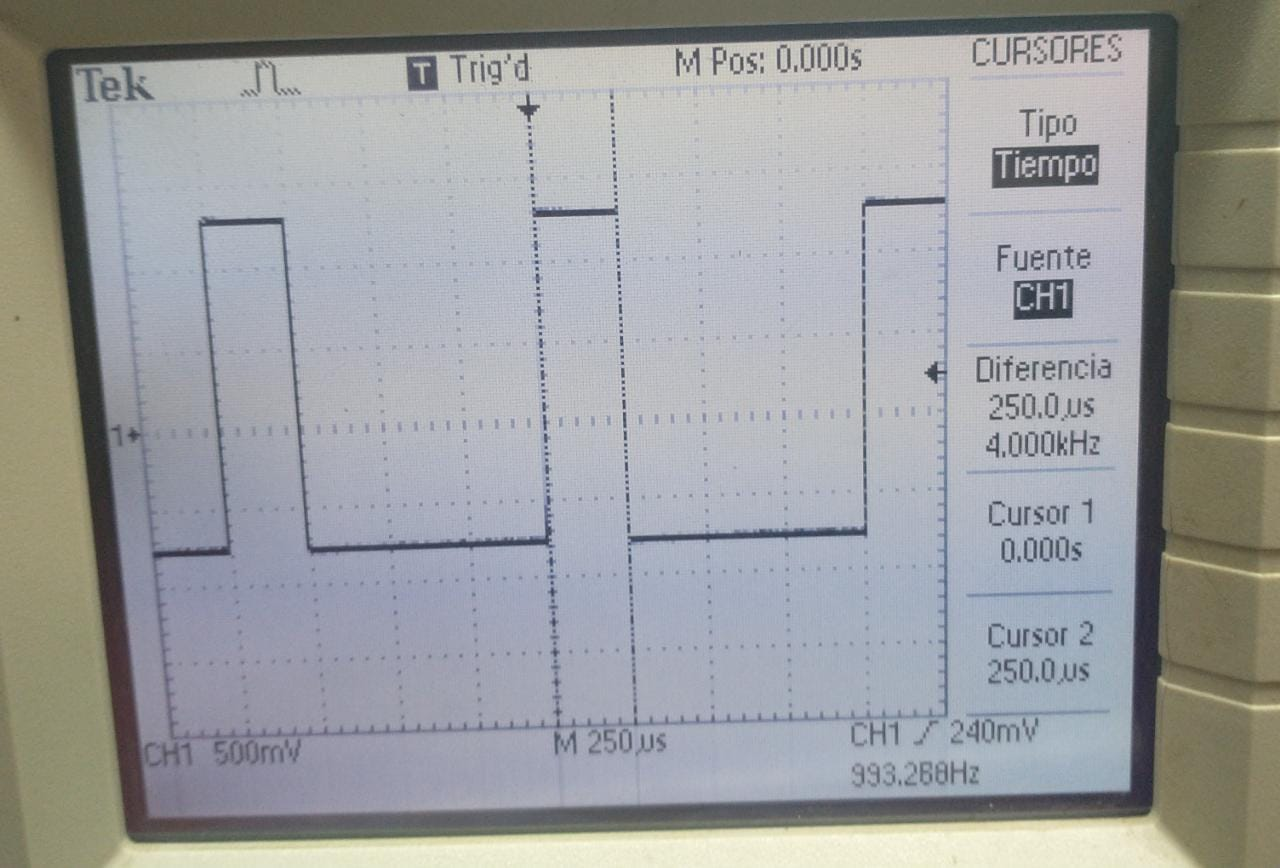
\includegraphics[width=\textwidth]{Imagenes/ActividadPractica/2AnalisisDeUnTrenDePulsos/Exp2_AnchoDelPulsoDeEntrada.jpeg}}
          \caption{Ancho del pulso de $250~\mu s$.}
        \end{subfigure}

        \caption{Tren de pulsos.}
        \label{fig:Exp2SeñalPulso}
      \end{figure}

    Ahora, se cambia al modo matemático a través del botón \textbf{MATH MENU}, y se configura con: \textbf{FFT}, 
    \textbf{CH1}, \textbf{Rectangular}, \textbf{Zoom X1} y modo adquisición \textbf{Promedio} en 64 muestras. 
    Dicha configuración se enseña en la Figura~\ref{fig:Exp2SeñalPulsanteEspectro}.

      \begin{figure}[H]
        \centering
          \frame{\includegraphics[width=0.48\textwidth]{Imagenes/ActividadPractica/2AnalisisDeUnTrenDePulsos/Exp2_EspectroDeLaSeñalPulsante.jpeg}}
          \caption{Análisis en frecuencia de la señal de entrada.}
          \label{fig:Exp2SeñalPulsanteEspectro}
      \end{figure}

      Luego, se observa cómo varía el espectro entre los 3 tipos de ventana: \textbf{Hanning}, \textbf{Rectangular}, 
      y \textbf{Flattop}, lo cual se ve en la Figura~\ref{fig:Exp2SeñalPulsanteVentanasEspectro}.

      \begin{figure}[H]
        \centering
        \begin{subfigure}[H]{0.48\textwidth}
          \frame{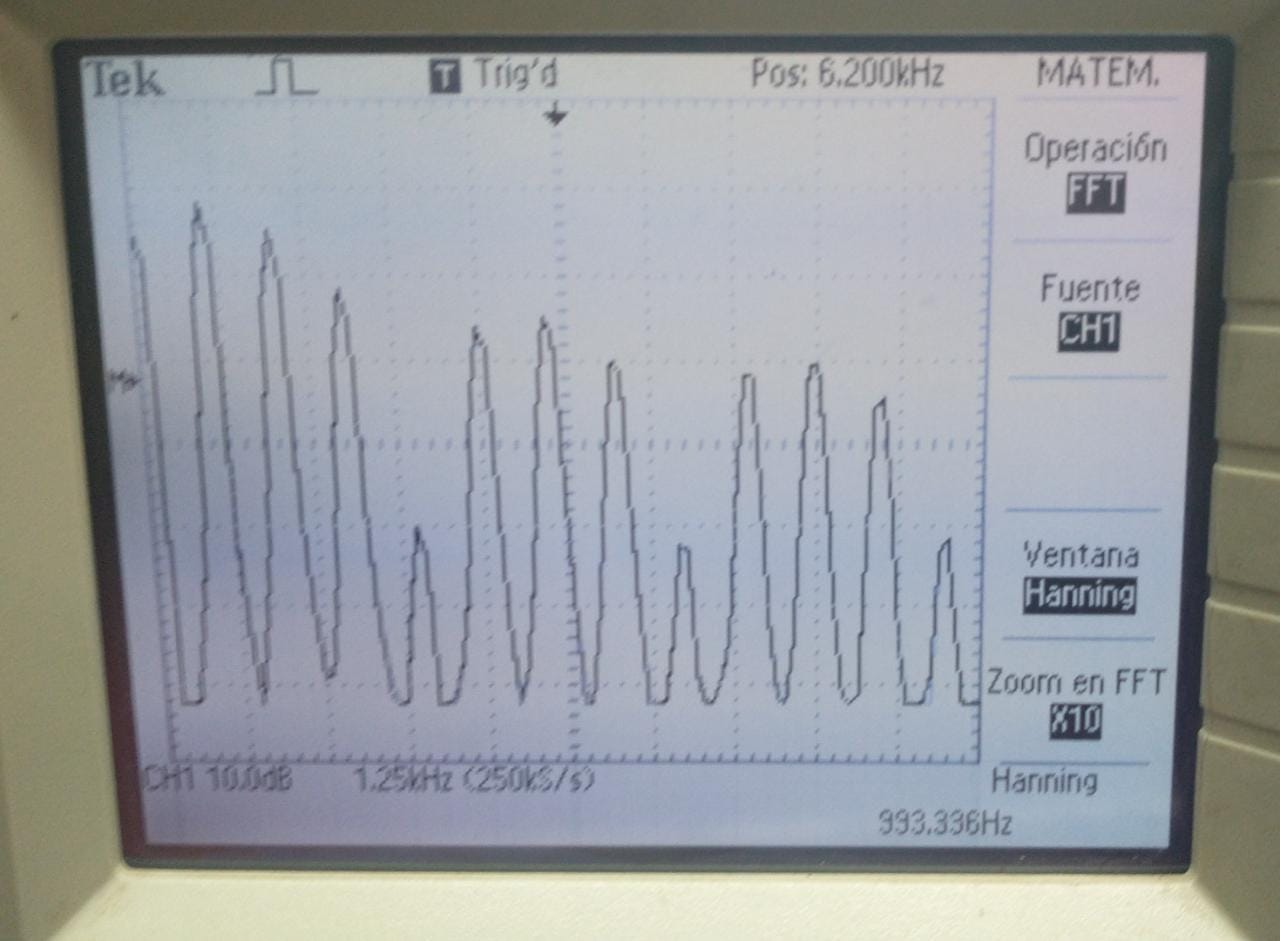
\includegraphics[width=\textwidth]{Imagenes/ActividadPractica/2AnalisisDeUnTrenDePulsos/Exp2_EspectroEnVentanaHannin.jpeg}}
          \caption{Ventana Hanning.}
        \end{subfigure}
        \hfill
        \begin{subfigure}[H]{0.48\textwidth}
          \frame{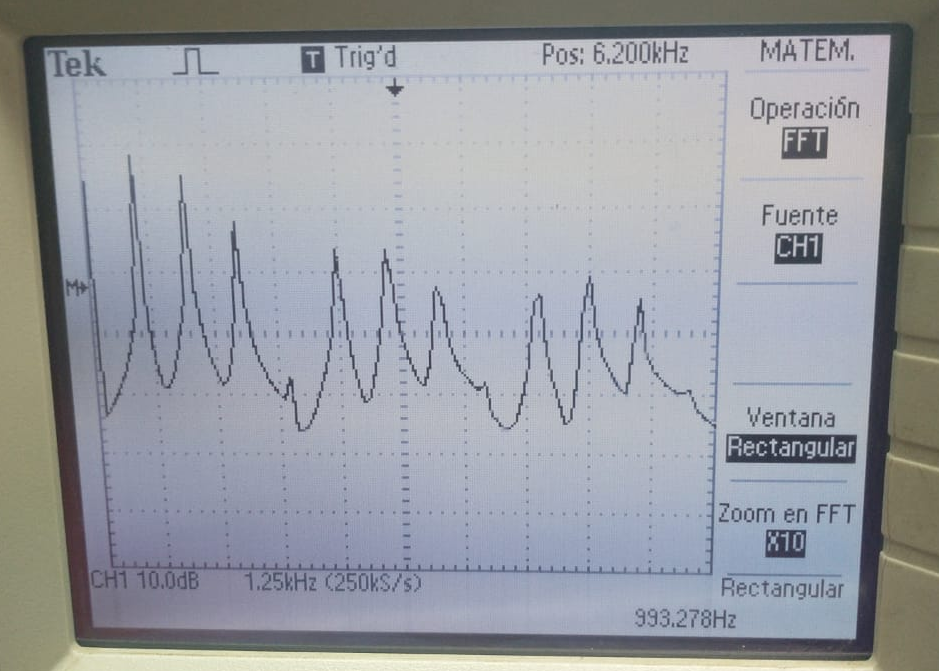
\includegraphics[width=\textwidth]{Imagenes/ActividadPractica/2AnalisisDeUnTrenDePulsos/Exp2_EspectroEnVentanaRectangular.png}}
          \caption{Ventana Rectangular.}
        \end{subfigure}
        \begin{subfigure}[H]{0.48\textwidth}
          \frame{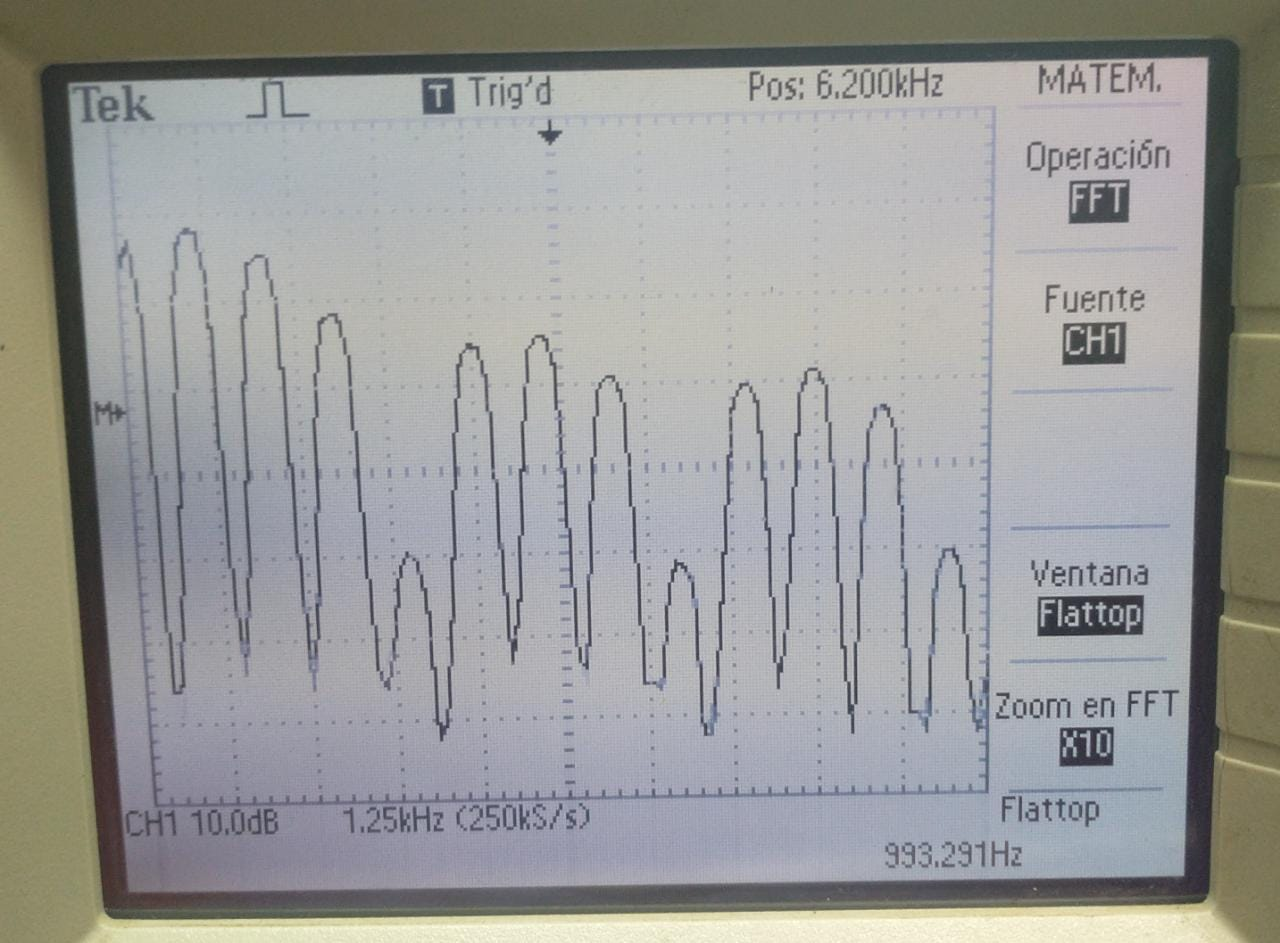
\includegraphics[width=\textwidth]{Imagenes/ActividadPractica/2AnalisisDeUnTrenDePulsos/Exp2_EspectroEnVentanaFlattop.jpeg}}
          \caption{Ventana Flattop.}
        \end{subfigure}

        \caption{Análisis en frecuencia con las distintas ventanas.}
        \label{fig:Exp2SeñalPulsanteVentanasEspectro}
      \end{figure}

      A continuación, se selecciona ventana \textbf{Rectangular}, se coloca el menú de cursores, y se selecciona 
      \textbf{frecuencia} en fuente 
      \textbf{Matemático}. Se coloca el \textbf{Cursor 1}, en $0~Hz$ y con el \textbf{Cursor 2} se 
      procede a medir las frecuencias de cada pico, como muestra la 
      Figura~\ref{fig:Exp2SeñalPulsanteArmonicosEspectro}.

       \begin{figure}[H]
        \centering
        \begin{subfigure}[H]{0.48\textwidth}
          \frame{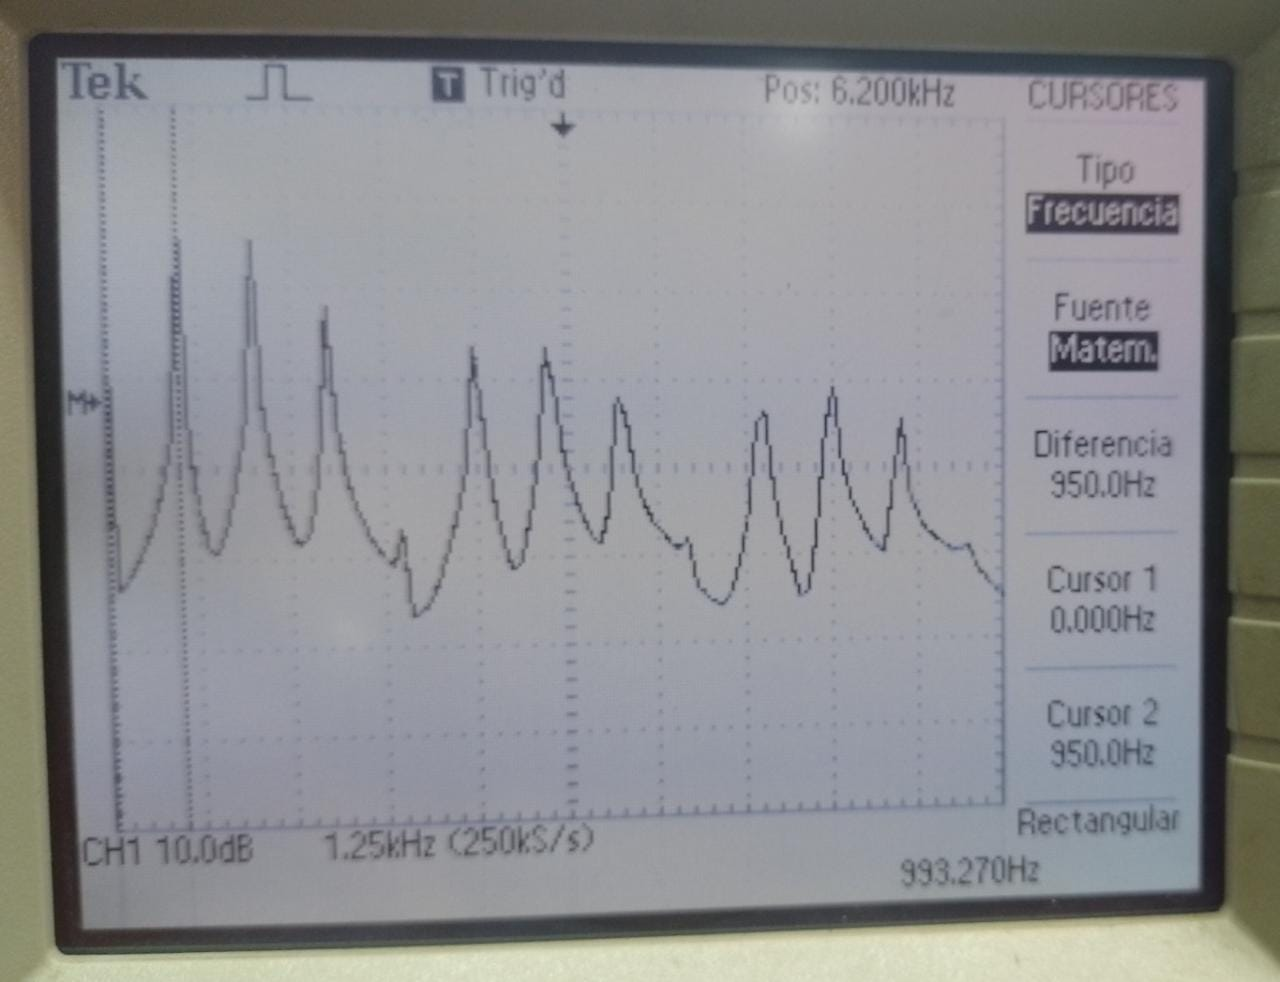
\includegraphics[width=\textwidth]{Imagenes/ActividadPractica/2AnalisisDeUnTrenDePulsos/Exp2_FrecArmonico1.jpeg}}
          \caption{Frecuencia de la fundamental en ventana Rectangular, $f_{1}=950~Hz$.}
        \end{subfigure}
        \hfill
        \begin{subfigure}[H]{0.48\textwidth}
          \frame{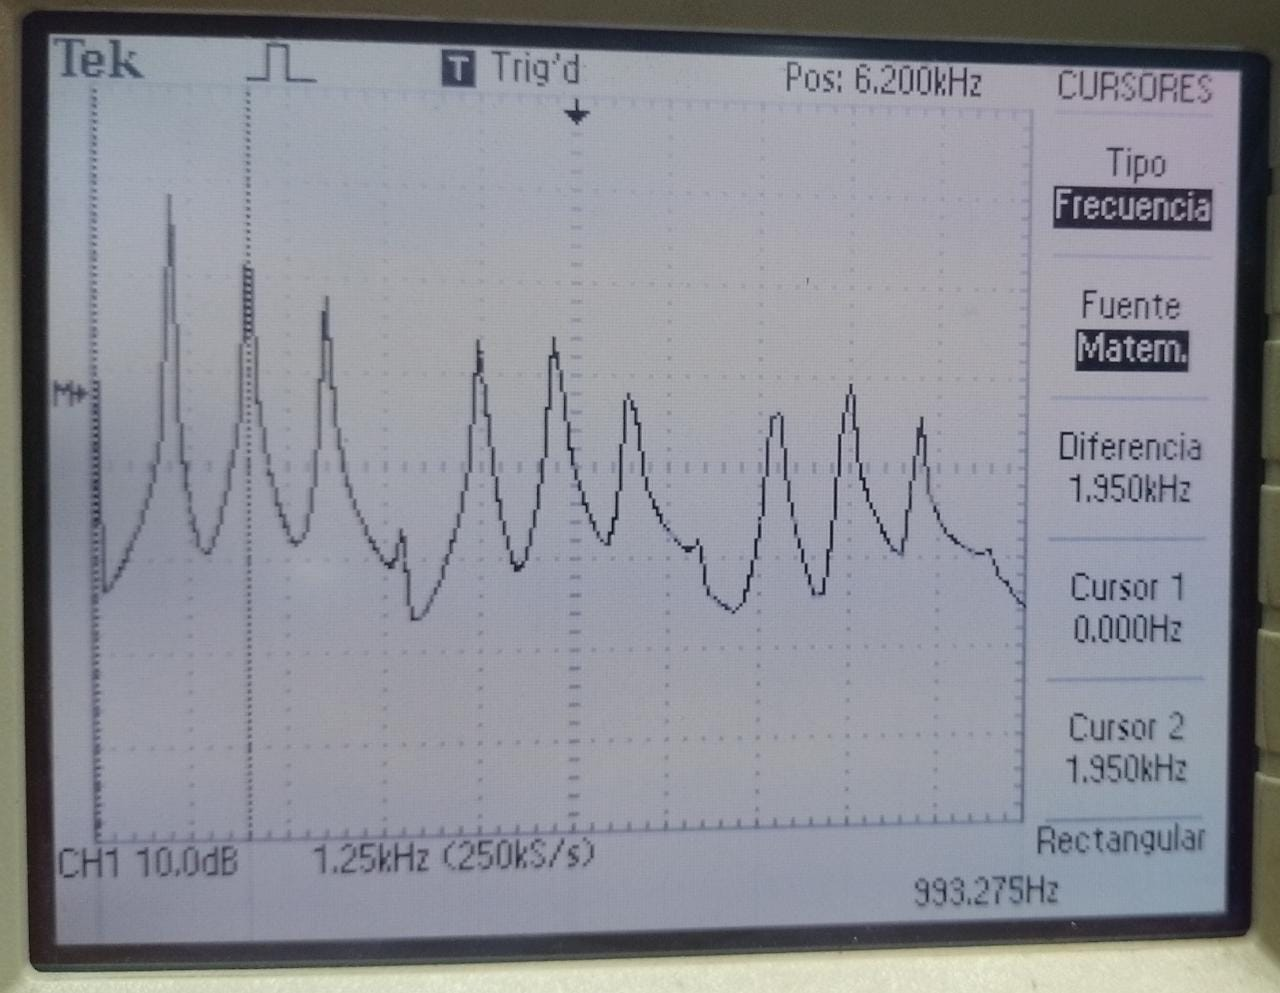
\includegraphics[width=\textwidth]{Imagenes/ActividadPractica/2AnalisisDeUnTrenDePulsos/Exp2_FrecArmonico2.jpeg}}
          \caption{Frecuencia de la segunda armónica en ventana Rectangular, $f_{2}=1950~Hz$.}
        \end{subfigure}
        \begin{subfigure}[H]{0.48\textwidth}
          \frame{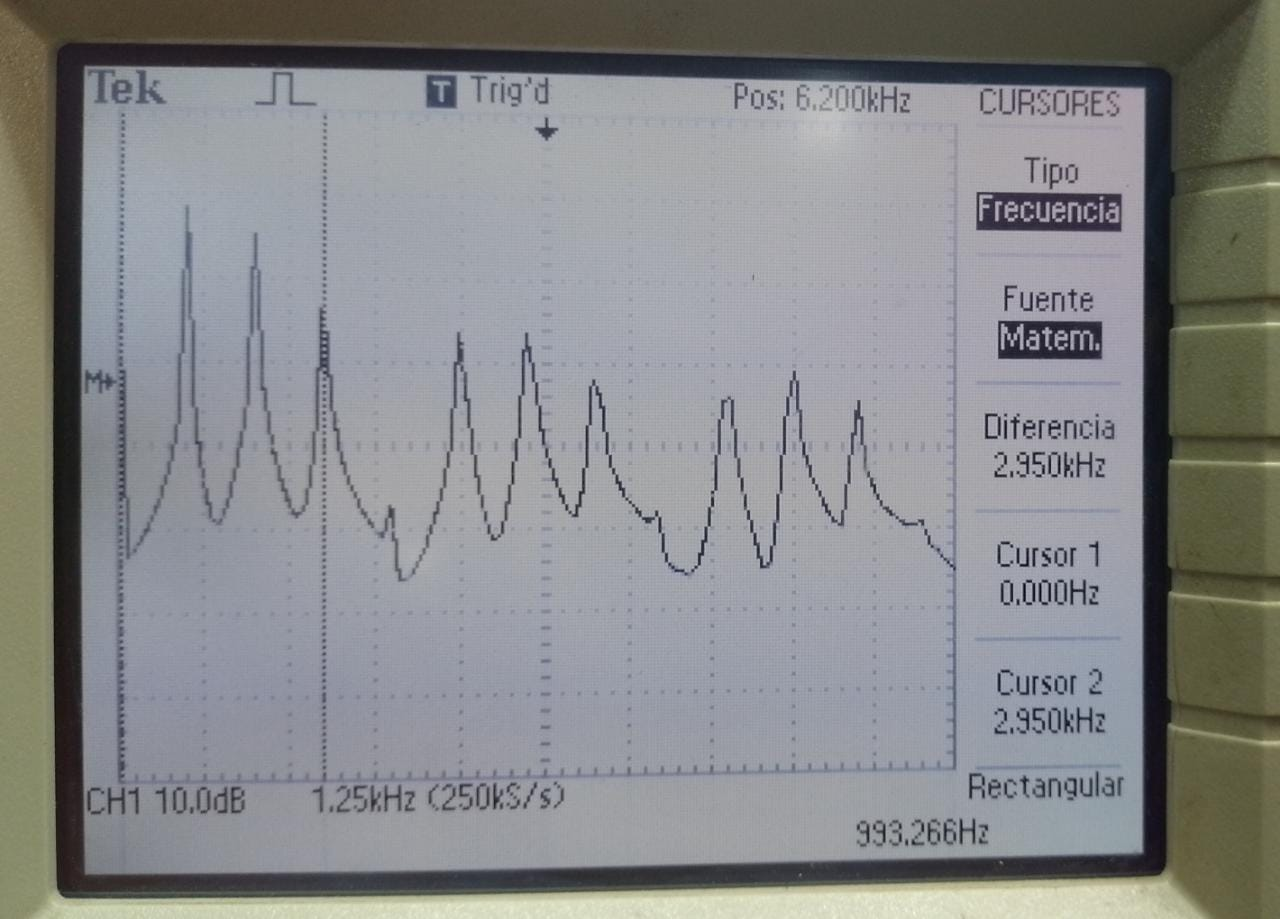
\includegraphics[width=\textwidth]{Imagenes/ActividadPractica/2AnalisisDeUnTrenDePulsos/Exp2_FrecArmonico3.jpeg}}
          \caption{Frecuencia de la tercera armónica en ventana Rectangular, $f_{3}=2950~Hz$.}
        \end{subfigure}
       \hfill
        \begin{subfigure}[H]{0.48\textwidth}
          \frame{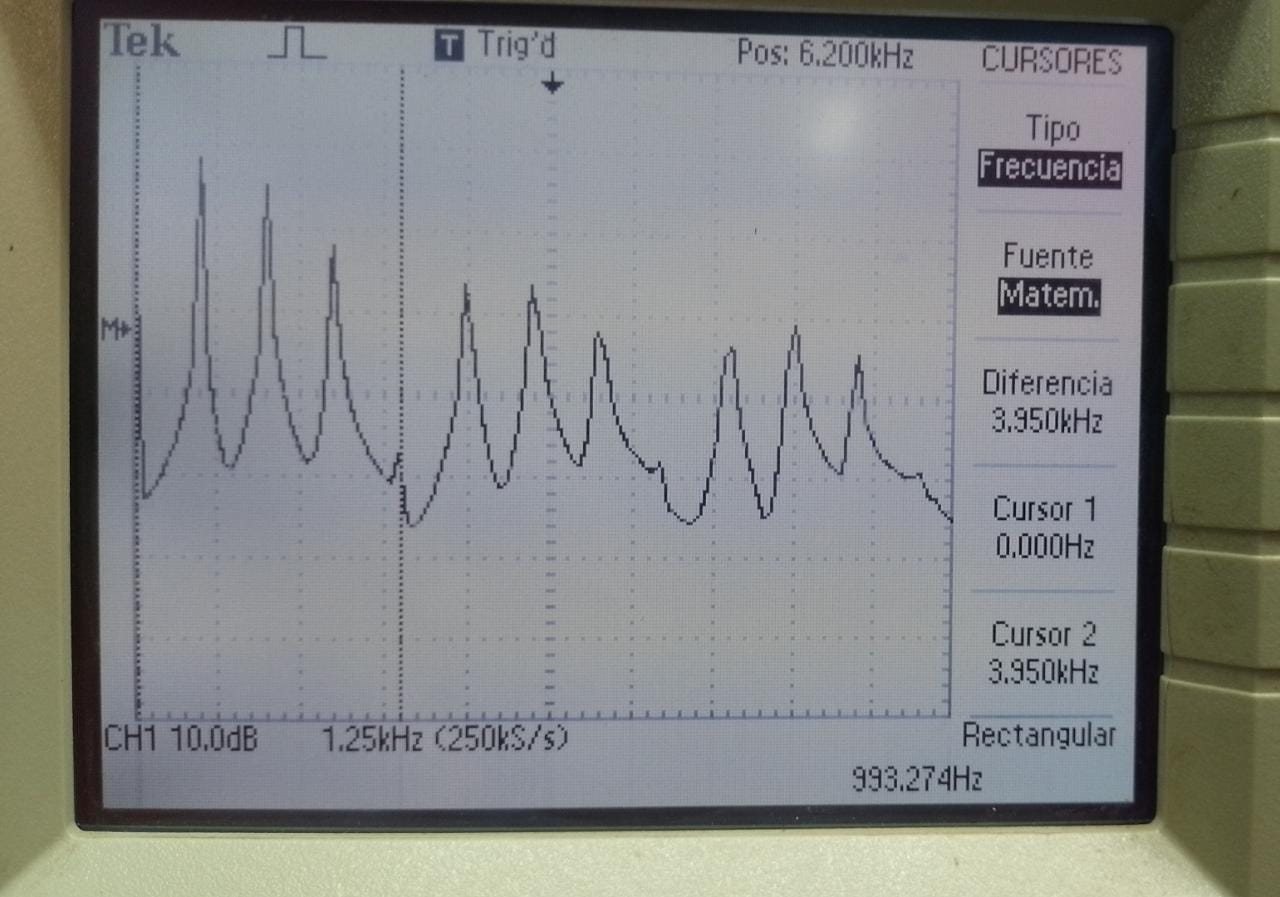
\includegraphics[width=\textwidth]{Imagenes/ActividadPractica/2AnalisisDeUnTrenDePulsos/Exp2_FrecArmonico4.jpeg}}
          \caption{Frecuencia de la cuarta armónica en ventana Rectangular, $f_{4}=3950~Hz$.}
        \end{subfigure}
        \begin{subfigure}[H]{0.48\textwidth}
          \frame{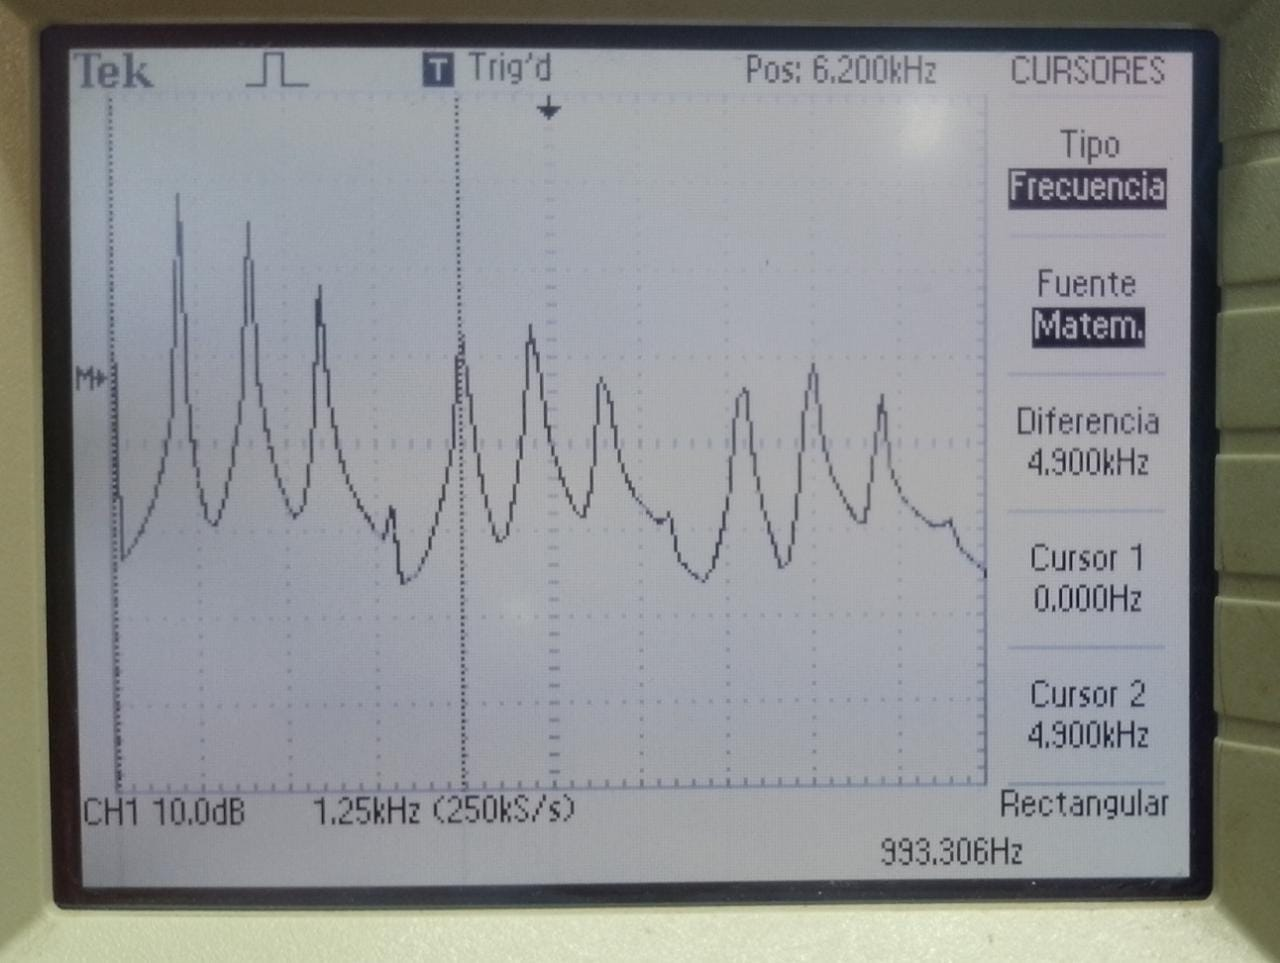
\includegraphics[width=\textwidth]{Imagenes/ActividadPractica/2AnalisisDeUnTrenDePulsos/Exp2_FrecArmonico5.jpeg}}
          \caption{Frecuencia de la quinta armónica en ventana Rectangular, $f_{5}=4900~Hz$.}
        \end{subfigure}

        \caption{Medición de frecuencia de picos de la señal pulsante en ventana Rectangular.}
        \label{fig:Exp2SeñalPulsanteArmonicosEspectro}
      \end{figure}     

      Se confecciona una tabla con las \textbf{diferencias de frecuencia} entre picos, en 
      base a las mediciones realizadas. Los valores se encuentran en la 
      Tabla~\ref{tab:Exp2MedicionesHanning}.

      \begin{table}[H]
      \centering
        \begin{tabular}{cccccc} \hline \hline
          \textbf{Cursor 2}               &  $\mathbf{1erArm.}$       & $\mathbf{2daArm.}$        & $\mathbf{3raArm.}$  &   $\mathbf{4taArm.}$ &   $\mathbf{5taArm.}$ \\ \hline
          $\mathbf{\Delta f_{n}~[Hz]}$     &   $950$                   &    $1000$                  &   $1000$             & $1000$                & $950$                \\ \hline \hline
         \end{tabular}
          \caption{Valores de frecuencia medidos en ventana Hanning.}
          \label{tab:Exp2MedicionesHanning}
      \end{table}

      Se calcula el promedio de las frecuencias como sigue
      \begin{align*}
        \Delta f_{n_{prom}}=\dfrac{\sum{\Delta_{fn}}}{n} \hspace{20pt} \therefore \hspace{20pt} \boxed{\Delta_{fn_{prom}}=980~[Hz]}~,
      \end{align*}
      y el período de la onda de pulsos es 
      \begin{align*}
        Periodo~\left( T \right)=\dfrac{1}{\Delta f_{n_{prom}}} \hspace{20pt} \therefore \hspace{20pt} \boxed{Periodo~\left( T \right)=1,02~[ms]}~.
      \end{align*}

        Se repite el experimento utilizando la ventana \textbf{Flattop}, pero ésta vez se miden los 
        \textbf{valles} que presenta el espectro, que se visualiza en la 
        Figura~\ref{fig:Exp2SeñalPulsanteVallesEspectro}.

       \begin{figure}[H]
        \centering
        \begin{subfigure}[H]{0.48\textwidth}
          \frame{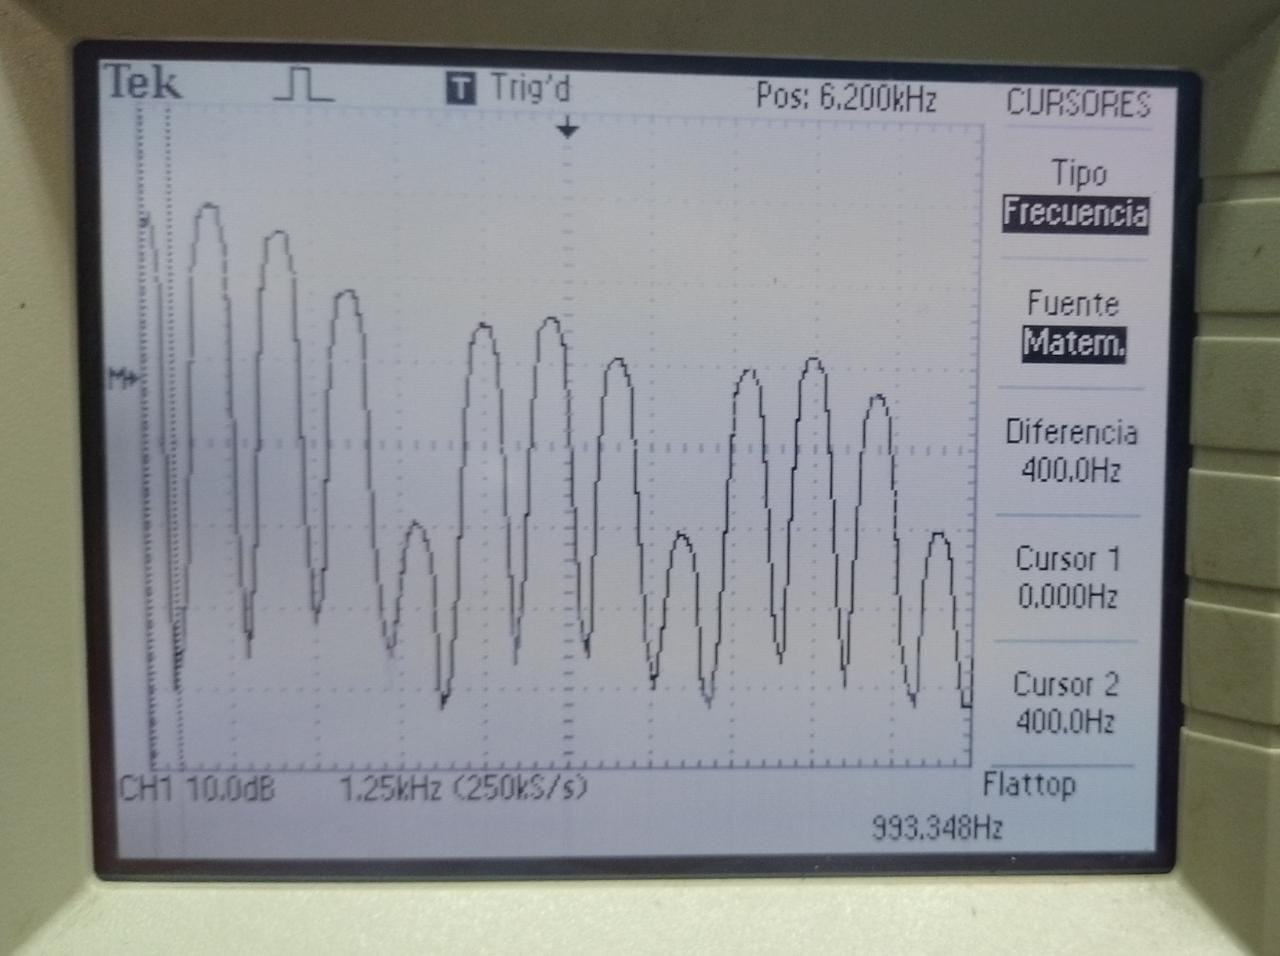
\includegraphics[width=\textwidth]{Imagenes/ActividadPractica/2AnalisisDeUnTrenDePulsos/Exp2_FrecValle1Flattop.jpeg}}
          \caption{Frecuencia del primer valle en ventana Flattop, $f_{a}=400~Hz$.}
        \end{subfigure}
        \hfill
        \begin{subfigure}[H]{0.48\textwidth}
          \frame{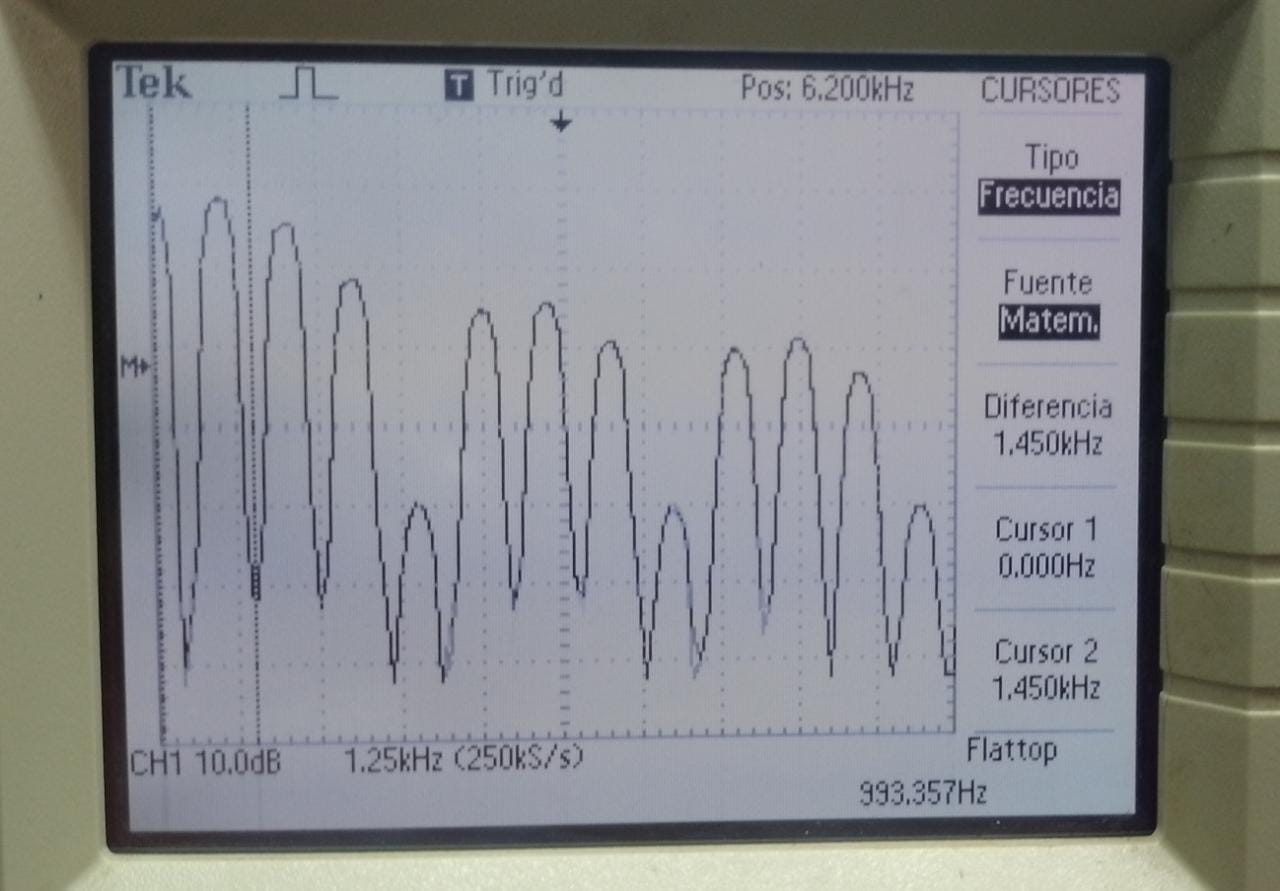
\includegraphics[width=\textwidth]{Imagenes/ActividadPractica/2AnalisisDeUnTrenDePulsos/Exp2_FrecValle2Flattop.jpeg}}
          \caption{Frecuencia del segundo valle en ventana Flattop, $f_{b}=1450~Hz$.}
        \end{subfigure}
        \hfill
        \begin{subfigure}[H]{0.48\textwidth}
          \frame{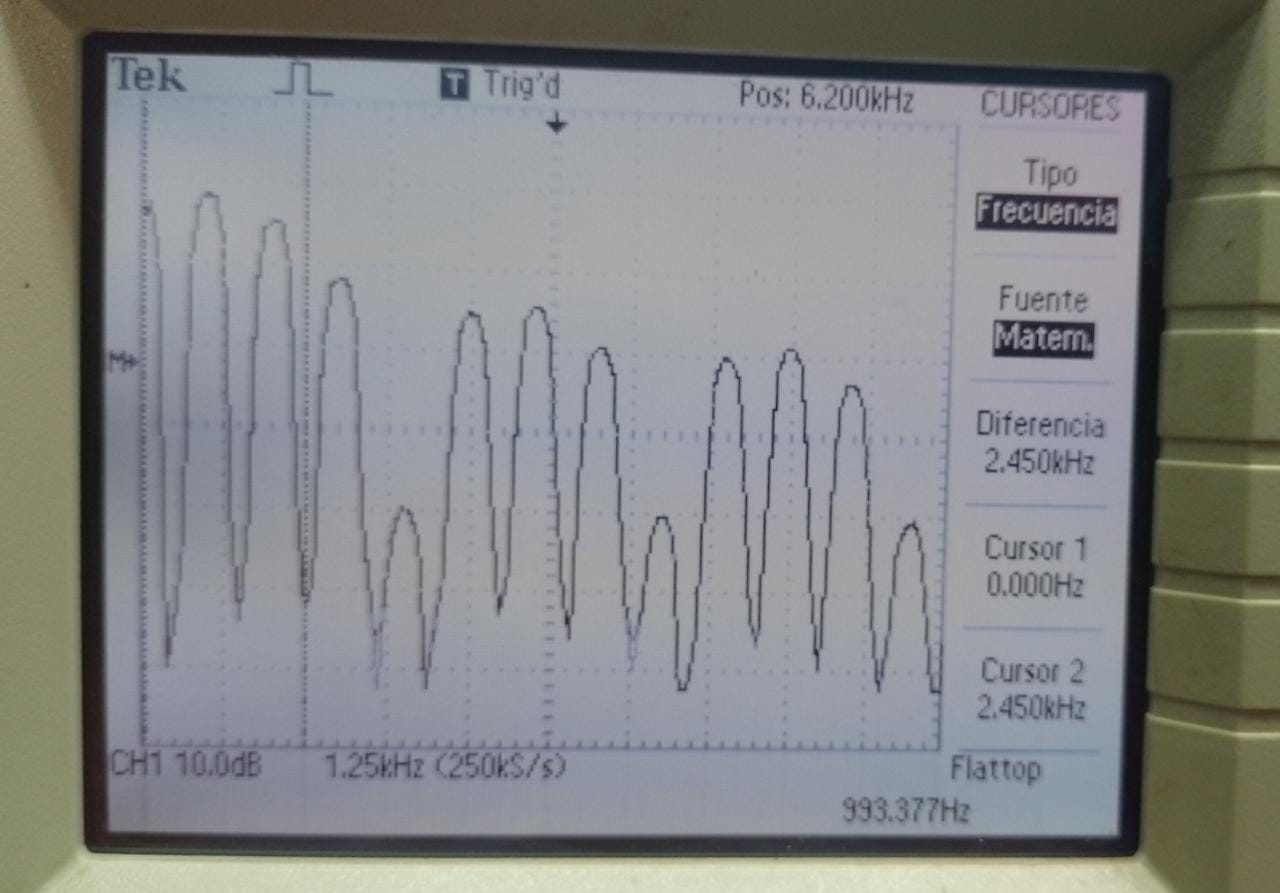
\includegraphics[width=\textwidth]{Imagenes/ActividadPractica/2AnalisisDeUnTrenDePulsos/Exp2_FrecValle3Flattop.jpeg}}
          \caption{Frecuencia del tercer valle en ventana Flattop, $f_{c}=2450~Hz$.}
        \end{subfigure}

        \caption{Medición de frecuencia de valles de la señal pulsante en ventana Flattop.}
        \label{fig:Exp2SeñalPulsanteVallesEspectro}
      \end{figure}     

      Se confecciona una tabla con los valores obtenidos, los mismos se encuentran en la 
      Tabla~\ref{tab:Exp2MedicionesFlattop}, y se calculan nuevamente el $\Delta f_{n_{prom}}$
      y el período. 

      \begin{table}[H]
      \centering
        \begin{tabular}{ccc} \hline \hline
          $\mathbf{\Delta_{fmin1}}$               &  $\mathbf{\Delta_{fmin2}}$       & $\mathbf{\Delta_{fmin3}}$ \\ \hline
                    $400~Hz$                        &    $1050~Hz$                    &   $1000~Hz$  \\ \hline \hline
         \end{tabular}
          \caption{Valores de frecuencia medidos en ventana Flattop.}
          \label{tab:Exp2MedicionesFlattop}
      \end{table}  

      \begin{align*}
        \Delta_{fn_{prom}}=\dfrac{\sum{\Delta_{fn}}}{n} \hspace{20pt} \therefore \hspace{20pt} \boxed{\Delta_{fn_{prom}}=816,67~[Hz]}
      \end{align*}        

      \begin{align*}
        Periodo~\left( T \right)=\dfrac{1}{\Delta_{fn_{prom}}} \hspace{20pt} \therefore \hspace{20pt} \boxed{Periodo~\left( T \right)=1,224~[ms]}
      \end{align*}

      Finalmente, se mide la amplitud de la frecuencia correspondiente a $0~Hz$, y se mide 
      también con multímetro el nivel de continua de la señal, posteriormente se comparan 
      los resultados.

       \begin{figure}[H]
        \centering
        \begin{subfigure}[H]{0.48\textwidth}
          \frame{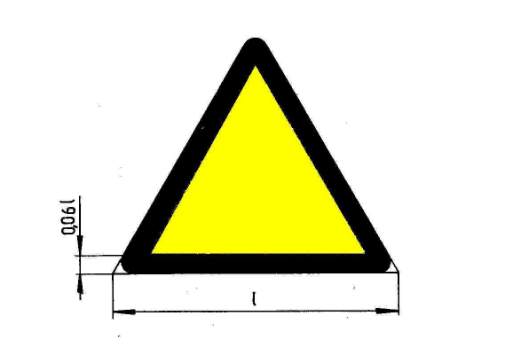
\includegraphics[width=\textwidth]{Imagenes/ActividadPractica/2AnalisisDeUnTrenDePulsos/ActPra_ejemplo.png}}
          \caption{Medición de continua con osciloscopio, $CC_{osc}=1~V$.}
        \end{subfigure}
        \hfill
        \begin{subfigure}[H]{0.48\textwidth}
          \frame{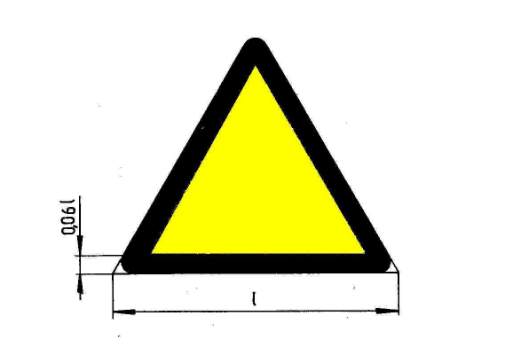
\includegraphics[width=\textwidth]{Imagenes/ActividadPractica/2AnalisisDeUnTrenDePulsos/ActPra_ejemplo.png}}
          \caption{Medición de continua con multímetro, $CC_{Mult}=1~V$.}
        \end{subfigure}

        \caption{Medición del nivel de continua de la señal pulsante.}
        \label{fig:Exp2SeñalPulsanteContinua}
      \end{figure}        
